\documentclass[a4paper,12pt]{article}
\usepackage[T1]{fontenc}
\usepackage[utf8]{inputenc}
\usepackage{polski}
\usepackage{color}
\usepackage{graphicx}
\usepackage{amsmath}
\usepackage{amssymb}
\usepackage{hyperref}
\usepackage{float}
\usepackage{listings}

\lstset{
  basicstyle=\ttfamily,
  columns=flexible,
  keepspaces=true,
  literate={ą}{{\k{a}}}1
           {ć}{{\'{c}}}1
           {ę}{{\k{e}}}1
           {ł}{{\l{}}}1
           {ń}{{\'{n}}}1
           {ó}{{\'{o}}}1
           {ś}{{\'{s}}}1
           {ź}{{\'{z}}}1
           {ż}{{\.{z}}}1
           {Ą}{{\k{A}}}1
           {Ć}{{\'{C}}}1
           {Ę}{{\k{E}}}1
           {Ł}{{\L{}}}1
           {Ń}{{\'{N}}}1
           {Ó}{{\'{O}}}1
           {Ś}{{\'{S}}}1
           {Ź}{{\'{Z}}}1
           {Ż}{{\.{Z}}}1
}

\title{2. sprawozdanie z laboratorium Hurtownie Danych}
\author{Mikołaj Kubś, 272662}
\date{\today}

\begin{document}

\maketitle

\section{Zadanie 1. Ekstrakcja danych}

\subsection{}

Utworzyć zestawienie, które dla poszczególnych miesięcy i lat przedstawi informację o liczbie różnych klientów. Przygotuj zapytanie z i bez użycia polecenia pivot.

\subsubsection{Wersja bez pivot}

\begin{lstlisting}[
    language=SQL,
    showspaces=false,
    basicstyle=\ttfamily,
    numbers=left,
    numberstyle=\tiny,
    commentstyle=\color{green}
    tabsize=2
    ]
SELECT 
YEAR(OrderDate), 
MONTH(OrderDate), 
COUNT(DISTINCT CustomerID) 
FROM Sales.SalesOrderHeader
GROUP BY YEAR(OrderDate), MONTH(OrderDate)
ORDER BY YEAR(OrderDate), MONTH(OrderDate)
\end{lstlisting}

\begin{figure}[H]
    \centering
    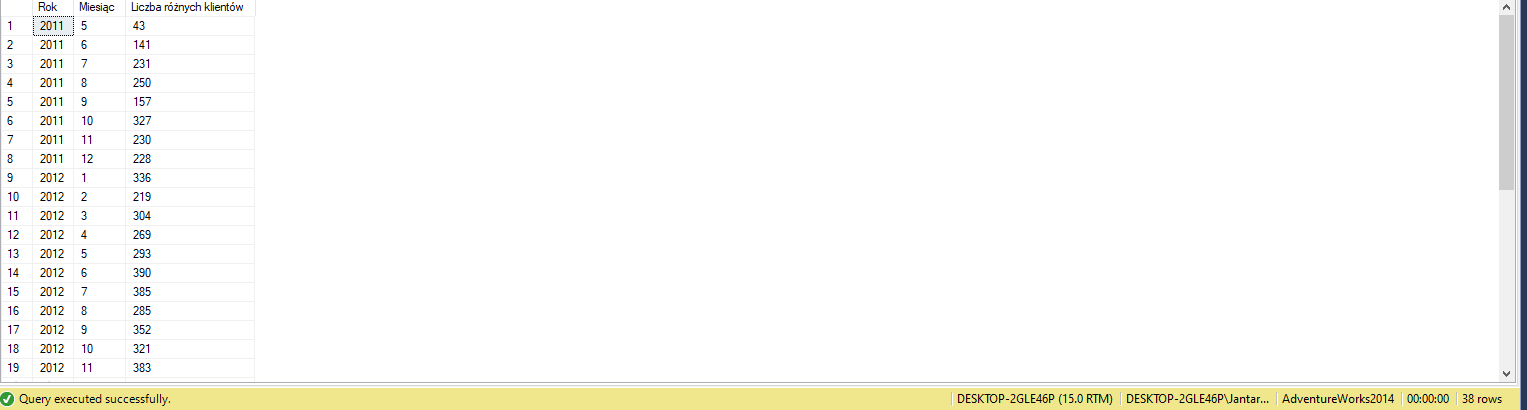
\includegraphics[width=0.8\textwidth]{images/01_normal.png}
    \caption{Wynik wykonania kwerendy 1}
    \label{fig:1_normal}
\end{figure}

\subsubsection{Wersja z użyciem pivot}

\begin{lstlisting}[
    language=SQL,
    showspaces=false,
    basicstyle=\ttfamily,
    numbers=left,
    numberstyle=\tiny,
    commentstyle=\color{green}
    tabsize=2
    ]
WITH UniqueCustomers AS (
    SELECT 
        YEAR(OrderDate) AS OrderYear, 
        MONTH(OrderDate) AS OrderMonth, 
        CustomerID
    FROM Sales.SalesOrderHeader
    GROUP BY YEAR(OrderDate), MONTH(OrderDate), CustomerID
)
SELECT * FROM UniqueCustomers
PIVOT (
    COUNT(CustomerID) 
    FOR OrderMonth IN ([1], [2], [3], [4], 
                       [5], [6], [7], [8], 
                       [9], [10], [11], [12])
) AS PivotTable
ORDER BY OrderYear;
\end{lstlisting}

\begin{figure}[H]
    \centering
    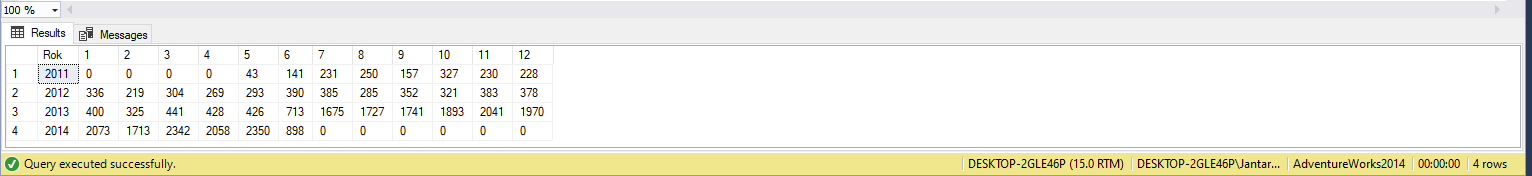
\includegraphics[width=0.8\textwidth]{images/01_pivot.png}
    \caption{Wynik wykonania kwerendy 1 z pivot}
    \label{fig:1_pivot}
\end{figure}

\subsection{}

Utworzyć zestawienie zawierające w wierszach imiona i nazwiska sprzedawców, a w kolumnach kolejne lata. Wartością będzie liczba obsłużonych transakcji. Wyświetlić tylko tych sprzedawców, którzy pracowali przez wszystkie 4 lata.

\begin{lstlisting}[
    language=SQL,
    showspaces=false,
    basicstyle=\ttfamily,
    numbers=left,
    numberstyle=\tiny,
    commentstyle=\color{green},
    tabsize=2
    ]
SELECT * FROM
(
	SELECT 
        FirstName, LastName, SalesOrderID, 
        YEAR(OrderDate) AS OrderYear FROM Sales.SalesPerson
	JOIN HumanResources.Employee ON 
        Employee.BusinessEntityID = SalesPerson.BusinessEntityID
	JOIN Person.Person ON 
        Person.BusinessEntityID = Employee.BusinessEntityID
	JOIN Sales.SalesOrderHeader ON 
        SalesOrderHeader.SalesPersonID = SalesPerson.BusinessEntityID
	WHERE YEAR(HireDate) = 2011
) AS SourceTable
PIVOT (
	COUNT(SalesOrderID)
	FOR OrderYear IN ([2011], [2012], [2013], [2014])
) AS PivotedTable
ORDER BY FirstName
\end{lstlisting}

\begin{figure}[H]
    \centering
    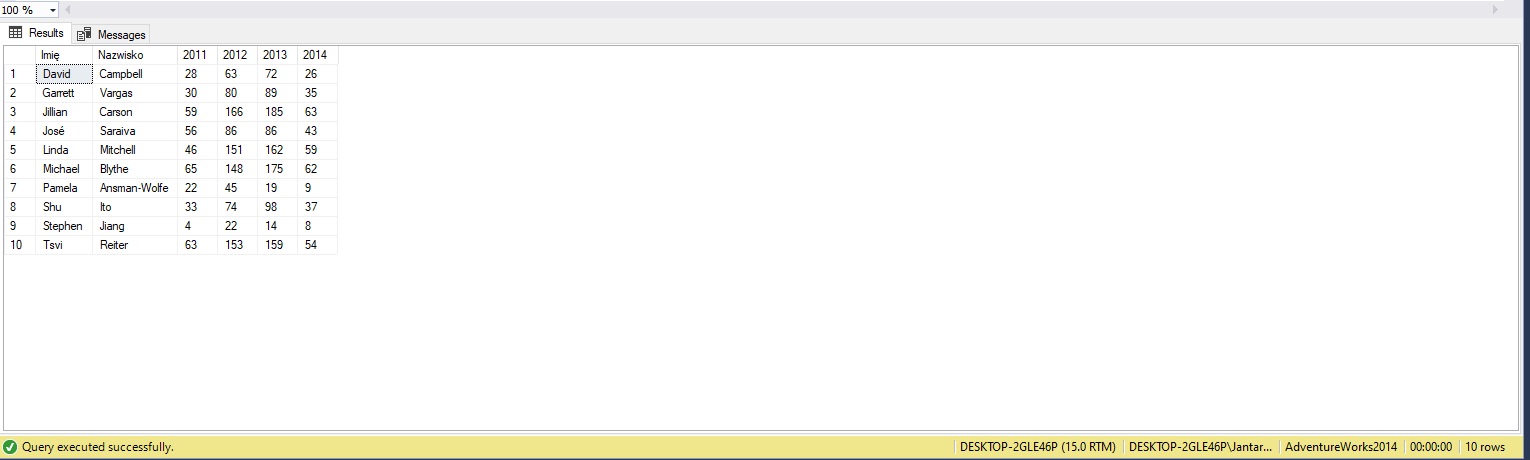
\includegraphics[width=0.8\textwidth]{images/02.png}
    \caption{Wynik wykonania kwerendy 2}
\end{figure}

\subsection{}

Zdefiniować zapytanie wyznaczające sumę kwot sprzedaży towarów oraz liczbę różnych produktów w zamówieniach w poszczególnych latach, miesiącach, dniach.

\begin{lstlisting}[
    language=SQL,
    showspaces=false,
    basicstyle=\ttfamily,
    numbers=left,
    numberstyle=\tiny,
    commentstyle=\color{green}
    tabsize=2
    ]
SELECT 
    YEAR(OrderDate) AS "Rok", 
    MONTH(OrderDate) AS "Miesiąc", 
    DAY(OrderDate) AS "Dzień", 
    SUM(LineTotal) AS "Suma", 
    COUNT(DISTINCT ProductID) AS "Liczba różnych produktów"
FROM Sales.SalesOrderHeader
JOIN Sales.SalesOrderDetail ON 
    SalesOrderDetail.SalesOrderID = SalesOrderHeader.SalesOrderID
GROUP BY YEAR(OrderDate), MONTH(OrderDate), DAY(OrderDate)
ORDER BY YEAR(OrderDate), MONTH(OrderDate), DAY(OrderDate)
\end{lstlisting}

\begin{figure}[H]
    \centering
    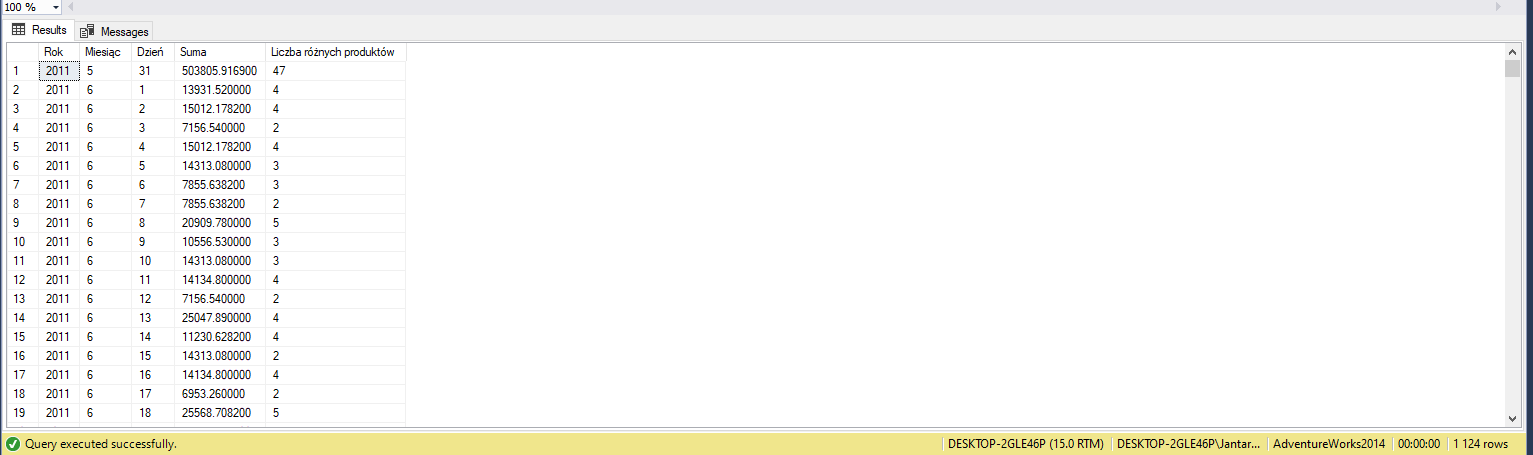
\includegraphics[width=0.8\textwidth]{images/03.png}
    \caption{Wynik wykonania kwerendy 3}
\end{figure}

\subsection{}

Wykorzystując polecenie CASE przygotować podsumowania do zestawienia z poprzedniego zadania tak, aby sumowane były kwoty zamówień oraz obliczana liczba różnych produktów dla poszczególnych miesięcy i dni tygodnia.\\
Uwaga: Pamiętaj o wybraniu właściwego atrybutu funkcji datepart tak, aby zgadzała się nazwa dnia tygodnia

\begin{lstlisting}[
    language=SQL,
    showspaces=false,
    basicstyle=\ttfamily,
    numbers=left,
    numberstyle=\tiny,
    commentstyle=\color{green}
    tabsize=2
    ]
SET DATEFIRST 1;
SET LANGUAGE Polish;

SELECT 
    YEAR(OrderDate) AS "Rok", 
    DATENAME(month, OrderDate) AS "Miesiąc",     
    CASE DATEPART(dw, OrderDate)
        WHEN 1 THEN 'Poniedziałek'
        WHEN 2 THEN 'Wtorek'
        WHEN 3 THEN 'Środa'
        WHEN 4 THEN 'Czwartek'
        WHEN 5 THEN 'Piątek'
        WHEN 6 THEN 'Sobota'
        WHEN 7 THEN 'Niedziela'
    END AS "Dzień tygodnia", 
    SUM(LineTotal) AS "Suma", 
    COUNT(DISTINCT ProductID) AS "Liczba różnych produktów"
FROM Sales.SalesOrderHeader
JOIN Sales.SalesOrderDetail ON 
    SalesOrderDetail.SalesOrderID = SalesOrderHeader.SalesOrderID
GROUP BY 
    YEAR(OrderDate), 
    DATENAME(month, OrderDate),
    MONTH(OrderDate),
    DATEPART(dw, OrderDate)
ORDER BY 
    YEAR(OrderDate), 
    MONTH(OrderDate), 
    DATEPART(dw, OrderDate)
\end{lstlisting}

\begin{figure}[H]
    \centering
    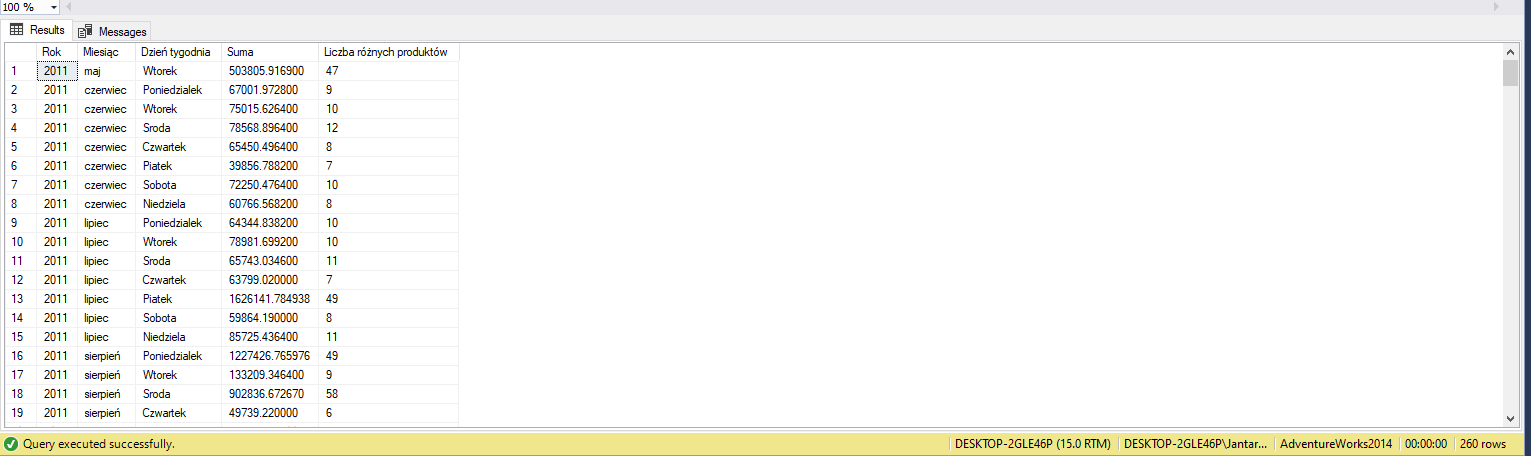
\includegraphics[width=0.8\textwidth]{images/04.png}
    \caption{Wynik wykonania kwerendy 4}
\end{figure}

\subsection{}

Przygotować zestawienie, w którym dla wybranych klientów przygotujemy kartę lojalnościową:\\
a. srebrną, jeśli klient wykonał co najmniej 2 transakcje w sklepie;\\
b. złotą, jeśli wykonał co najmniej 4 transakcje w sklepie, w tym co najmniej 2 transakcje, których łączna kwota przekraczała 250\% średniej wartości zamówień w bazie;\\
c. platynową, jeśli klient spełniał warunki otrzymania karty złotej oraz w co najmniej jednej transakcji kupił jednocześnie produkty ze wszystkich kategorii

\begin{lstlisting}[
    language=SQL,
    showspaces=false,
    basicstyle=\ttfamily,
    numbers=left,
    numberstyle=\tiny,
    commentstyle=\color{green}
    tabsize=2
    ]
WITH AvgOrderValue AS (
    SELECT AVG(TotalOrderValue) AS AvgValue
    FROM (
        SELECT SalesOrderID, SUM(LineTotal) AS TotalOrderValue
        FROM Sales.SalesOrderDetail
        GROUP BY SalesOrderID
    ) AS OrderValues
),
CustomerOrders AS (
    SELECT 
        SOH.CustomerID, 
        COUNT(DISTINCT SOH.SalesOrderID) AS TransactionCount, 
        SUM(SOD.LineTotal) AS TotalTransactionValue, 
        SUM(CASE WHEN OrderValues.TotalOrderValue > 2.5 * A.AvgValue
            THEN 1 ELSE 0 END)AS HighValueOrderCount
    FROM Sales.SalesOrderHeader SOH
    JOIN Sales.SalesOrderDetail SOD ON SOD.SalesOrderID = SOH.SalesOrderID
    JOIN (
        SELECT SalesOrderID, SUM(LineTotal) AS TotalOrderValue
        FROM Sales.SalesOrderDetail
        GROUP BY SalesOrderID
    ) AS OrderValues ON SOH.SalesOrderID = OrderValues.SalesOrderID
    CROSS JOIN AvgOrderValue A 
    GROUP BY SOH.CustomerID
),
UniqueCategories AS (
    SELECT 
        C.CustomerID, 
        COUNT(DISTINCT PC.ProductCategoryID) AS CategoryCount
    FROM Sales.Customer C
    JOIN Sales.SalesOrderHeader SOH ON SOH.CustomerID = C.CustomerID
    JOIN Sales.SalesOrderDetail SOD ON SOD.SalesOrderID = SOH.SalesOrderID
    JOIN Production.Product PR ON PR.ProductID = SOD.ProductID
    JOIN Production.ProductSubcategory PSC ON 
        PSC.ProductSubcategoryID = PR.ProductSubcategoryID
    JOIN Production.ProductCategory PC 
        ON PC.ProductCategoryID = PSC.ProductCategoryID
    GROUP BY C.CustomerID
)
SELECT 
    P.FirstName AS "Imię",
    P.LastName AS "Nazwisko",
    COALESCE(CO.TransactionCount, 0) AS "Liczba transakcji",
    COALESCE(CO.TotalTransactionValue, 0) AS "Łączna kwota transakcji",
    CASE 
        WHEN CO.TransactionCount >= 4 
            AND CO.HighValueOrderCount >= 2 
            AND COALESCE(UC.CategoryCount, 0) = 
                (SELECT COUNT(*) FROM Production.ProductCategory) 
            THEN 'Platynowa'
        WHEN CO.TransactionCount >= 4 
            AND CO.HighValueOrderCount >= 2 
            THEN 'Złota'
        WHEN CO.TransactionCount >= 2 
            THEN 'Srebrna'
        ELSE 'Brak karty'
    END AS "Kolor karty"
FROM Sales.Customer C
LEFT JOIN CustomerOrders CO ON CO.CustomerID = C.CustomerID
LEFT JOIN UniqueCategories UC ON UC.CustomerID = C.CustomerID
JOIN Person.Person P ON P.BusinessEntityID = C.CustomerID
ORDER BY CO.TransactionCount DESC;    
\end{lstlisting}

\begin{figure}[H]
    \centering
    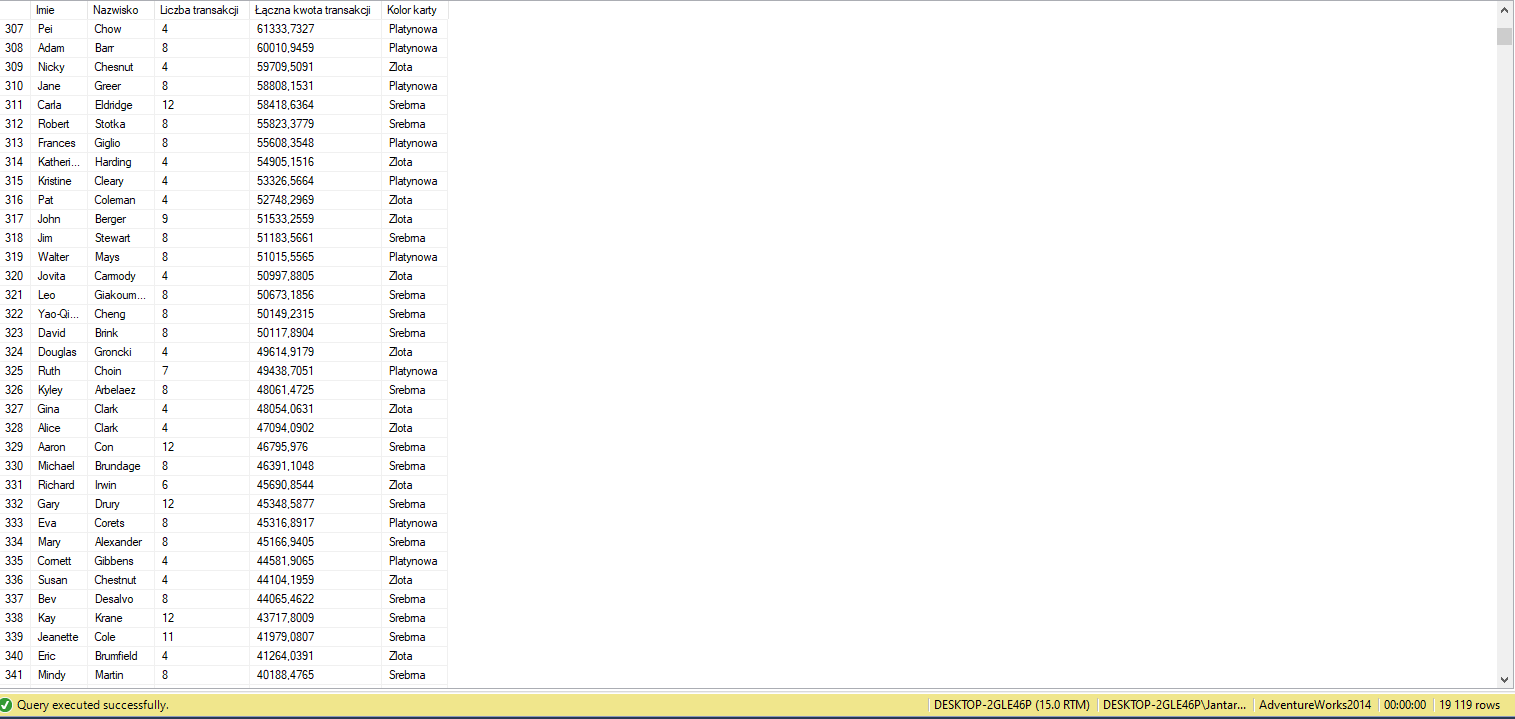
\includegraphics[width=0.8\textwidth]{images/05.png}
    \caption{Wynik wykonania kwerendy 5}
\end{figure}

\end{document}